%%
%% in order to compile this source the `ACM Master Article Template'
%% must be installed in your latex distribution (or in your Overleaf
%% environment)
%% https://www.acm.org/publications/proceedings-template
%%
%% If you have specific questions related to this package please refer
%% to the User Documentation:
%% https://www.acm.org/binaries/content/assets/publications/consolidated-tex-template/acmart.pdf
%%
\documentclass[acmsmall,nonacm]{acmart}

%% start of the body of the document source.
\begin{document}

%% ===========================================================================
%% === Title =================================================================
%% ===========================================================================
%% The "title" command has an optional parameter,
%% allowing the author to define a "short title" to be used in page headers.
\title[Short Title Here]{Review: Include Title of Assigned Paper Here}

%% ===========================================================================
%% === Authors ===============================================================
%% ===========================================================================
%% The "author" command and its associated commands are used to define
%% the authors and their affiliations.
%% Of note is the shared affiliation of the first two authors
\author{Name LastName}
\email{email@institution.edu}
\orcid{1234-5678-9012} % optional
% this author shares institution with the next author 
% thus affiliation is not required

\author{John Johns}
\email{webmaster@institution.edu}
\affiliation{%
    \institution{Institute for Clarity in Documentation}
    \streetaddress{P.O. Box 1212}
    \city{Dublin}
    \state{Ohio}
    \postcode{43017-6221}
}

\author{Ruby Pascal}
\affiliation{%
    \institution{Programming University}
    \streetaddress{Loop 12}
    \city{Mountain View}
    \state{CA}
    \country{USA}
}

%% ===========================================================================
%% === Abstract ==============================================================
%% ===========================================================================
\begin{abstract}
    This document introduces general guidelines for writing paper reviews for ``CSC 592: Neural Networks and Deep Learning''. This template is based on the ACM Master Article Template, the same used by ACM in conference proceedings or journal publication. All students are strongly encouraged to use the provided \LaTeX\ source to generate the paper review.
\end{abstract}

%% ===========================================================================
%% === Create the Title ======================================================
%% ===========================================================================
%% This command processes the author and affiliation and title
%% information and builds the first part of the formatted document.
\maketitle

%% ===========================================================================
%% === Introduction ==========================================================
%% ===========================================================================
\section{Introduction}

In this class you will be required to read a number of papers.  The goal is that you gain experience in reading and evaluating academic papers.  Expect to spend 2-3 hours reading the paper and 1-2 hours writing a review.  If you are not used to read scientific publications, this time can take longer initially.  Due dates for paper reviews are posted on the course website.  As indicated in the syllabus, {\bf no late submissions will be accepted}.

You are strongly encouraged to use this template to write your review.  We are providing the compiled (PDF) and source files (sources and figures) to replicate this file.  If you don't have a current \LaTeX\ distribution in your computer you can use a free web service such as Overleaf~\footnote{www.overleaf.com}.  If you are using a local distribution, make sure you have installed the ``\verb|acmart|'' package.  This package can be used to prepare articles for any ACM publication --- conference or journal, and for any stage
of publication, from review to final ``camera-ready'' copy, to the
author's own version, with {\it very} few changes to the source.

For further information about the ``\verb|acmart|'' package, the {\LaTeX\ User's Guide} available at \url{https://www.acm.org/publications/proceedings-template}, provides a complete explanation of commands and tips for their effective use.

%% ===========================================================================
%% === Writing a Paper Review ================================================
%% ===========================================================================
\section{Writing a Paper Review}

After thoroughly reading the assigned paper, you are expected to write a single document containing the structure described in Table~\ref{tab:structure}.
 
\begin{table}[h!]
    \caption{Recommended structure for a paper review}
    \label{tab:structure}
    \begin{tabular}{lcc}
        \toprule
        Section title & Expected length & Points \\
        \midrule
        Summary & $1/2$ page & $35$ pts \\
        Critique & $1/2$ page & $25$ pts \\
        Insights & $1/2$ page & $20$ pts \\
        Future Work & $1/2$ page & $20$ pts \\
        \bottomrule
    \end{tabular}
\end{table}

\subsection{Summary}
The summary provides a high level description of the paper.  Some of the questions below can be used to guide your writing:
\begin{itemize}
    \item What is the research problem the paper attempts to address?
    \item What are the claimed contributions of the paper?
    \item How do the authors substantiate their claims?
    \item What are the main takeaways from the results presented in the paper?
\end{itemize}

\subsection{Critique}
In this section you will provide an itemized list of strengths followed by another of weaknesses.  When trying to identify strengths and weaknesses, you can analyze as many of the following points as possible: introduction, contributions, significance/importance, related work, methodology, experiments/analysis, conclusion, writing style.

\subsection{Insights gained}
In this section you will present a description of the most relevant aspects/topics you have learned after reading this paper.

\subsection{Future work}
Propose one or two ways in which the research work can be further developed. Do not repeat the {\it Future Work} section of the paper.

%% ===========================================================================
%% === Submission ============================================================
%% ===========================================================================
\section{How to submit your reviews?}
For each assigned paper you will submit a corresponding paper review as a single PDF file.  All submissions are done via Gradescope.  Once you upload your PDF to Gradescope, you will be asked to mark which pages of your PDF correspond to questions of the assignment.  For each question, mark the pages containing the answer by first clicking on a question on the left and then clicking on the corresponding page(s) on the right.  Further information about Gradescope submissions is available at \url{https://www.gradescope.com/help#help-center-item-student-submitting}.

%% ===========================================================================
%% === Additional Resources ==================================================
%% ===========================================================================
\section{Additional Resources}
The following sections provide additional resources for reading papers and writing your document with \LaTeX.

\subsection{On reading academic papers}
If this is the first time that you are reading an academic paper, you are strongly encouraged to read the following resources before completing your first paper review:

\begin{itemize}
    \item Reading a Computer Science Research Paper~\cite{Fong-2009}
    \item How to Read a Paper~\cite{Keshav-2007}
\end{itemize}

\subsection{Including mathematical formulas}
A formula that appears in the running text is called an inline or in-text formula.  It can be produced by using \verb|$.$|.  For example, \verb|$y=\sigma\left(\mathbf{w}^T\mathbf{x}\right)$| will produce $y=\sigma\left(\mathbf{w}^T\mathbf{x}\right)$.  You can also use the \verb|displaymath| environment to display equations separated from the text, as the example below:
\begin{displaymath}
    \frac{\partial L}{\partial w_i} = \frac{\partial z}{\partial w_i} \frac{\partial L}{\partial z}
\end{displaymath}

\subsection{Figures}
Figures can be included and automatically referenced in the text using the \verb|includegraphics| and \verb|ref| commands, respectively.  Inspect the \LaTeX\ code provided with this document for more details on how to include the picture shown in Figure~\ref{f:roadster}.

\begin{figure}[h!]
    \centering
    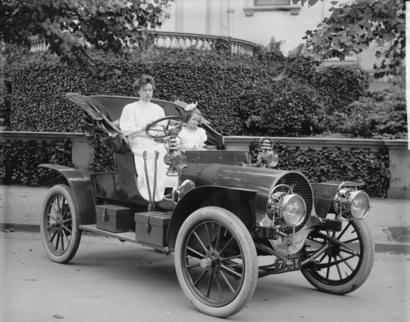
\includegraphics[width=4in]{sample}
    \caption{1907 Franklin Model D roadster. Photograph by Harris \& Ewing, Inc. [Public domain], via Wikimedia Commons.}
    \label{f:roadster}
\end{figure}

\subsection{Compiling \LaTeX\ code}
To compile a \LaTeX\ source into a PDF file, you can perform the following sequences of commands in your terminal.
\begin{verbatim}
    pdflatex document
    bibtex document
    pdflatex document
    pdflatex document
\end{verbatim}

%% The next two lines define the bibliography style to be used, and
%% the bibliography file.
\bibliographystyle{ACM-Reference-Format}
% references indicates that all references are stored in a file (in the 
% same folder as the latex source) named `references.bib`
\bibliography{references} 

\end{document}
\endinput
